The choice of the right controller is essential for robotics applications and usually goes hand in hand with the choice of the hardware platform.
There are controllers that can provide precision in the range of micrometers, and others that can compliantly interact with the environment.
For this work, the latter case is much more relevant, since the investigated tactile manipulation skills interact with the environment in potentially complex ways.
In the following the rigid body dynamics
\begin{equation}
{\massmatrix}(\q)\ddq+{\coriolis}(\q,\dq)\dq+\gravityvector(\q)=\torqued+\exttorque,
\end{equation}
is considered, where ${\massmatrix}(\q)$ is the symmetric, positive definite mass matrix, $\coriolis(\q,\dq)$ the Coriolis matrix, $\V{g}(\q)$ the gravity vector, $\exttorque$ the vector of external link-side joint torques and $\torqued$ a controller joint-torque command.

\subsubsection{Impedance Control}

Impedance control aims to control the motion of a robot as well as its interaction behavior with the environment.
A typical formulation for a rigid, $n$-DOF manipulator in Cartesian space is given by
\begin{equation}
\torqued=\jacobian(\q)^T(\stiffnesscart \V{e} - \dampingcart \dot{\V{e}})) + \torque_r
\end{equation}

where $\stiffnesscart$ is the Cartesian stiffness matrix, $\dampingcart$ is the damping matrix and $\jacobian(\q)$ is the Jacobian.
The position and velocity errors are denoted by $\V{e}=\V{x}^\star - \V{x}$ and $\dot{\V{e}}=\dot{\V{x}}^\star - \dot{\V{x}}$, respectively.
The dynamics compensator $\torque_r(t)$ can be defined in multiple ways, see for example \cite{Yang.2011}.
The Cartesian damping matrix requires design e.g. according to \cite{AlbuSchaffer.2003}.

Note that
\begin{equation}
\stiffness \V{e} + \damping \dot{\V{e}} + [M_x \ddot{\V{e}}]
\end{equation}

defines the desired interaction dynamics of the robot with the environment.
The last term would determine the desired inertia, however, due to the difficulty of measuring or estimating the acceleration in real-world systems, it is usually left out. Note though that this is a topic of current research efforts \cite{birjandi2020observer}.
\\
Impedance control was first introduced to robotics in \cite{Hogan.661984681984,Hogan.1985,Hogan.1985b}.
Since then much work has been done to explore the numerous possibilities and variations of this control scheme.
In \cite{Anderson.1988} force information was used in addition to improve impedance control for uncertain environment as in deburring, grinding, and assembly tasks.
\cite{Hogan.1987} showcases an impedance controller implementation which is able to switch between free motion and a contact task, without having to use inverse kinematic computations.
In \cite{Lawrence.1988} an analysis of stability properties is provided focusing on two main implementations of impedance control.
In \cite{Schneider.1989} an object-centric impedance controller was introduced, which compensates the system's dynamics and directly controls the internal forces of a grasped object.

Especially the Cartesian space formulation of impedance control has been extensively researched, e.g. in \cite{AlbuSchaffer.2002} where impedance control is compared to admittance and stiffness control and a new impedance controller enhanced by local stiffness control was proposed.
In \cite{AlbuSchaffer.2003} several practical aspects of impedance control are discussed such as nullspace stiffness for redundant manipulators, avoidance of mass matrix decoupling and damping design.
\cite{Jung.2004} introduces a force-tracking impedance controller able to track a desired force in the presence of uncertainties in the environment as well as in the robot dynamic model.
The results were demonstrated in simulation and real-world experiments.
In \cite{Ferretti.2004} impedance control has been applied to 6-DOF industrial robots in several experiments.
In \cite{Duchaine.2007} a velocity based variable impedance controller is tested for human-robot cooperation using force differentiation to determine human intention.
The authors of \cite{AlbuSchaffer.2007} describe a general passivity-based framework for the control of flexible joint robots that incorporates position, torque and impedance control.
In \cite{Ott.2008} two impedance controllers for flexible joint robots are proposed based on an inner torque feedback loop.
\cite{Ott.2008b} provides a thorough overview of Cartesian impedance control for redundant and flexible-joint robots.
In \cite{Buchli.2011} an application of reinforcement learning for learning variable impedance control is demonstrated in simulation and real-world experiments.
Current surveys on impedance control can be found in \cite{Song.2017,Song.2019}.

Although single-arm manipulators have been one of the driving factors in impedance control research, the scheme has been successfully applied to various other fields.
In \cite{Ibarra.2014} applications to lower-limb rehabilitation can be found.
Also for hydraulic \cite{Ha.2000,Koivumaki.2017} and pneumatic \cite{Toedtheide.2016,Toedtheide.2017} actuators impedance control schemes have been developed.
Other areas where impedance control has assumed a central role are whole-body control for wheeled \cite{Dietrich.2011,Dietrich.2016,Bussmann.2018} and biped humanoids \cite{Rocchi.2015,Vorndamme.2016,Koivumaki.2017}, UAVs \cite{Lippiello.2012}, exoskeletons \cite{Khan.2015,Li.2017}, telepresence \cite{Love.2004,Nuno.2008,Tufail.2014}, and multi-fingered hands \cite{Wimbock.2011}.

\subsubsection{Adaptive Impedance Control}

Early work on adaptive impedance control can be found e.g. in \cite{Carelli.1991,kelly1989adaptive}.
The authors of \cite{Ikeura.1995} introduced a variable impedance controller for cooperation tasks between robots and humans.
They first analyzed the human behavior in a human-human tasks and then encoded the results in their controller model.
In \cite{Colbaugh.1993} an adaptive impedance controller was introduced which consists of a filter component, an adaptive controller, and an algorithm that maps the Cartesian-space control input to the joint-space control torque.
The controller does not require knowledge of the robot's dynamics parameters or the inverse kinematics.
In \cite{Kamnik.1998} model reference adaptive control was applied to impedance control and demonstrated on an industrial robot.
The authors of \cite{Cheah.1998} applied an iterative learning scheme to impedance control on a SCARA robot.
\cite{sharifi2014nonlinear} introduces, tests and compares for nonlinear adaptive impedance controllers for human-robot interaction.
Inspired by human motor control \cite{Burdet.2001}, the impedance control methodology has been extended to adaptive versions where the stiffness (and possibly damping) and an additional feedforward wrench are dependent on the tracking error \cite{Ganesh.2010,Yang.2011,Ganesh.2012}.
The exact behavior is governed by a learning factor and a forgetting factor.
Such an adaptive impedance controller is given by
\begin{equation*}
        \torqued=\jacobian(\q)(-\wrenchff(t)-\wrenchd(t)-\stiffnesscart(t)\boldsymbol{e}-\dampingcart[\massmatrix(\q),\boldsymbol{K}(t,\boldsymbol{K})] \dot{\boldsymbol{e}})
\end{equation*}
where $\wrenchff(t)$ is the adaptive feedforward wrench, $\wrenchd(t)$ is an additional predefined wrench trajectory that encodes potential prior knowledge, and $\stiffnesscart(t)$ is the adaptive stiffness matrix.
The approach was also extended to a deformable environment \cite{li2018force}.

\subsubsection{Force Control}

A typical force controller in Cartesian space can be expressed by
\begin{equation}
\torqued=\jacobian(\q)^T(\V{k}_p \V{f}_e + \V{k}_i \int_0^t (\wrenchd(\sigma)-\extwrench(\sigma))d\sigma + \V{k}_d \dot{\V{f}}_e )
\end{equation}

where $\V{k}_p$ is the proportional gain, $\V{k}_i$ is the integral gain, $\V{k}_d$ is the derivative gain of the control law, and $\V{f}_e=\wrenchd-\extwrench$ is the force error.

Force control is e.g. used in unmodeled contact situations or if the goal of a task requires precise (even dynamic) force tracking.

Force control in robotics has been researched for many years now.
In \cite{Khatib.1986} a method for combining motion control and force control has been presented based on the operational space formulation.
\cite{Whitney.1987} provides an early (historical) review of force control in robotics.
The authors of \cite{Eppinger.1986,Eppinger.1987} provide insights into the role of dynamics and nonlinearities in force control approaches.
In \cite{Eom.1998} a force control scheme without force sensor based on a disturbance observer is presented and demonstrated in a real-world experiment.
\cite{Roy.2002} introduces an adaptive force control algorithm for velocity and position controlled robot arms.
Force control has been applied in many robotics-related areas. The authors of \cite{Cortesao.2017} presented an observer-supported force controller that is able to compensate the motion of a beating heart, thus aiding cardiac interventions. In \cite{Stephens.2010} a controller to track desired contact forces for whole-body approaches in humanoids is presented. Other research focuses on contact forces in human-robot collaborations \cite{Magrini.2015} or surface electromyogram-based control strategies for exoskeletons \cite{Li.2014}.
Most force controller schemes rely on external force/torque sensors or joint torque sensors and a momentum observer \cite{Haddadin.2017}. Others have also shown approaches without force sensing \cite{Stolt.2012}.
Some earlier surveys can be found in \cite{Zeng.1997,Siciliano.1999,Yoshikawa.2000}.

\subsubsection{Unified Force / Impedance Control}

Unified force / impedance control combines the advantages of force control and impedance control in a single controller.
Early work can be found in \cite{almeida1999force} that enables impedance control and position-limited force control simultaneously.
\cite{schindlbeck2015unified} introduces a unified controller connected to an energy tank that preserves passivity of the system.
This approach was extended in \cite{karacan2022passivity}.
\cite{marin2016unified} presents a force / impedance control augmented with a kinestatic filter, which ensures that the commanded pose and wrench are consistent with a given task model.
\cite{lin2021unified} proposes a unified motion / force / impedance controller for unknown contacts.

A unified force/impedance controller can be written as
\begin{equation}
    \torqued=-\jacobian\left[\boldsymbol{k}_p (\wrenchd-\extwrench)+\boldsymbol{k}_d (\dwrenchd-\dot{\extwrench})+\boldsymbol{k}_i \boldsymbol{h}_i(\extwrench,t) +\stiffnesscart \boldsymbol{e} + \dampingcart \dot{\boldsymbol{e}}\right]
\end{equation}
where $\stiffnesscart$ is the Cartesian stiffness matrix, $\dampingcart$ is the Cartesian damping matrix, $\boldsymbol{k}_p$, $\boldsymbol{k}_d$, and $\boldsymbol{k}_i$ are the force controller gains, and $\boldsymbol{h}_i$ is defined as
\begin{equation}
    \boldsymbol{h}_i(\extwrench,t)=\int_0^t (\wrenchd(\sigma)-\extwrench(\sigma))d\sigma
\end{equation}

% \subsubsection{Safety}

% Robot safety is not a research subject of this thesis, however, there are many aspects associated with it that play an important role in the developed methods.

% The goal of making robots safe for humans has been pursued for some time now \cite{Hirschfeld.1993,Traver.2000,Lim.2000} but only in the last two decades some breakthroughs were made that made safety a major topic.
% This was especially driven by the emergence of lightweight, collaborative robots \cite{Hirzinger.2002}.
% In \cite{EdColgate.2008} a survey on pHRI can be found reviewing the relevant technologies and methodologies at that time.
% In \cite{Luca.2005} a method to detect collisions along a robot's structure without the use of acceleration or force measurements was developed.
% In \cite{Luca.2007} a collision detection methodology based on total energy and generalized momentum was proposed and demonstrated on a real robot.
% The authors of \cite{Haddadin.2008} developed a framework of collision detection and reaction methods for safe human-robot collaboration.
% Important works in the industrial and collaborative contexts are for example \cite{Haddadin.2009b} where insights into crash tests with robots are given, \cite{Haddadin.2009} where several robots were evaluated regarding the influence of their mass and velocity on injuries and \cite{Haddadin.2012} where a safe motion unit was developed which takes into account medical injury data to bound the velocity of the robot.
% In \cite{Vasic.2013} a survey of safety issues in industrial robotics, with autonomous mobile robots in human-inhabited areas, and with assistive robots.
% In \cite{Lacevic.2013} a danger field is proposed which indicates the current danger level with respect to the robot's pose and velocity.
% It can also be used to shape internal control schemes to make the motions of the robot safer.
% Collision handling was also applied to other areas of robotics, such as humanoids \cite{Vorndamme.2016,Vorndamme.2017} or UAVs \cite{Tomic.91420149182014}.
% In \cite{Haddadin.2017}, a recent survey on collision detection, isolation and identification can be found.
% It proposes an in general valid collision event pipeline with seven phases, see Fig \ref{fig:related:safety}.

% \begin{figure}[h!]
% 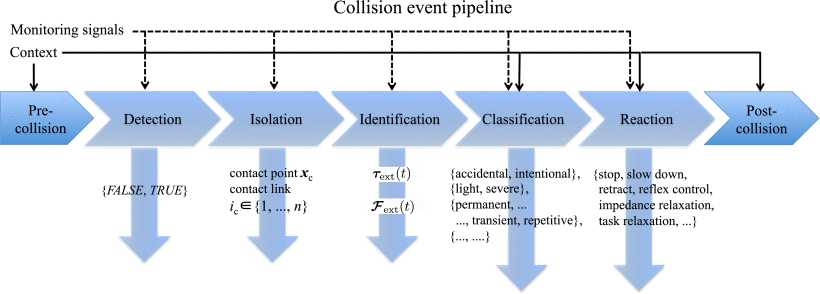
\includegraphics[width=\textwidth]{figures/related_safety.jpg}
% \caption{Seven phases of the collision event pipeline \cite{Haddadin.2017}}
% \label{fig:related:safety}
% \end{figure}

% Safety also plays an important role for robot learning where the main challenge is the right compromise between safety constraints and policy demands.
% Examples are \cite{Akametalu.2014} where a Gaussian process-based method is proposed to integrate safety and learning and \cite{Fisac.2019} where a safety framework for reinforcement learning methods was introduced and experimentally validated on a drone.
% In \cite{SpencerM.Richards.2018} a neural network Lyapunov function is developed which adapts a policy to a safe subset of the state space during learning.
% The method is demonstrated on a simulated inverted pendulum.
% \cite{Hewing.2020} a review of learning-based model predictive control is provided.

% \cite{Tadele.2014} provides a review on safety-related work for domestic robots.
% The authors of \cite{Guiochet.2017} review established safety paradigms in light of current robot technology.
% In \cite{Villani.2018b} a current survey is provided with a focus on human-robot collaboration in industrial environments.




